\chapter{Diseño e implementación} % Main chapter title

En este capítulo se describe la arquitectura en detalle de la solución. Se presenta una breve introducción a los patrones de software utilizados con especial foco en las técnicas de concurrencia. El trabajo realizado utiliza la plataforma de hardware EDU-CIAA, la API desarrollada bajo el nombre de Firmware_v3, y el sistema operativo de tiempo real FreeRTOS.\\

Siguiendo los lineamientos del marco de trabajo en ingeniería de software, se presentan los requerimientos, las funcionalidades y los casos de uso principales como ejes del espacio problema. Para describir el espacio solución se presenta la arquitectura, patrones, firmware y planos del hardware en el resto de las secciones.\\


\label{Chapter3} % Change X to a consecutive number; for referencing this chapter elsewhere, use \ref{ChapterX}

\definecolor{mygreen}{rgb}{0,0.6,0}
\definecolor{mygray}{rgb}{0.5,0.5,0.5}
\definecolor{mymauve}{rgb}{0.58,0,0.82}

%%%%%%%%%%%%%%%%%%%%%%%%%%%%%%%%%%%%%%%%%%%%%%%%%%%%%%%%%%%%%%%%%%%%%%%%%%%%%
% parámetros para configurar el formato del código en los entornos lstlisting
%%%%%%%%%%%%%%%%%%%%%%%%%%%%%%%%%%%%%%%%%%%%%%%%%%%%%%%%%%%%%%%%%%%%%%%%%%%%%
\lstset{ %
  backgroundcolor=\color{white},   % choose the background color; you must add \usepackage{color} or \usepackage{xcolor}
  basicstyle=\footnotesize,        % the size of the fonts that are used for the code
  breakatwhitespace=false,         % sets if automatic breaks should only happen at whitespace
  breaklines=true,                 % sets automatic line breaking
  captionpos=b,                    % sets the caption-position to bottom
  commentstyle=\color{mygreen},    % comment style
  deletekeywords={...},            % if you want to delete keywords from the given language
  %escapeinside={\%*}{*)},          % if you want to add LaTeX within your code
  %extendedchars=true,              % lets you use non-ASCII characters; for 8-bits encodings only, does not work with UTF-8
  %frame=single,	                % adds a frame around the code
  keepspaces=true,                 % keeps spaces in text, useful for keeping indentation of code (possibly needs columns=flexible)
  keywordstyle=\color{blue},       % keyword style
  language=[ANSI]C,                % the language of the code
  %otherkeywords={*,...},           % if you want to add more keywords to the set
  numbers=left,                    % where to put the line-numbers; possible values are (none, left, right)
  numbersep=5pt,                   % how far the line-numbers are from the code
  numberstyle=\tiny\color{mygray}, % the style that is used for the line-numbers
  rulecolor=\color{black},         % if not set, the frame-color may be changed on line-breaks within not-black text (e.g. comments (green here))
  showspaces=false,                % show spaces everywhere adding particular underscores; it overrides 'showstringspaces'
  showstringspaces=false,          % underline spaces within strings only
  showtabs=false,                  % show tabs within strings adding particular underscores
  stepnumber=1,                    % the step between two line-numbers. If it's 1, each line will be numbered
  stringstyle=\color{mymauve},     % string literal style
  tabsize=2,	                   % sets default tabsize to 2 spaces
  title=\lstname,                  % show the filename of files included with \lstinputlisting; also try caption instead of title
  morecomment=[s]{/*}{*/}
}


A modo de ejemplo:

\begin{lstlisting}[label=cod:vControl,caption=Pseudocódigo del lazo principal de control.]  % Start your code-block

#define MAX_SENSOR_NUMBER 3
#define MAX_ALARM_NUMBER  6
#define MAX_ACTUATOR_NUMBER 6

uint32_t sensorValue[MAX_SENSOR_NUMBER];		
FunctionalState alarmControl[MAX_ALARM_NUMBER];	//ENABLE or DISABLE
state_t alarmState[MAX_ALARM_NUMBER];						//ON or OFF
state_t actuatorState[MAX_ACTUATOR_NUMBER];			//ON or OFF

void vControl() {

	initGlobalVariables();
	
	period = 500 ms;
		
	while(1) {

		ticks = xTaskGetTickCount();
		
		updateSensors();
		
		updateAlarms();
		
		controlActuators();
		
		vTaskDelayUntil(&ticks, period);
	}
}
\end{lstlisting}



\section{Requerimientos}

\pagebreak
\section{Casos de Uso}

\pagebreak

\section{Arquitectura}

\subsection{Contexto}
\begin{figure}[ht]
	\centering
	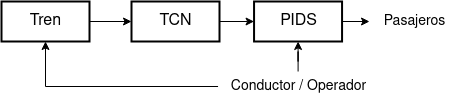
\includegraphics[width=1\textwidth]{./Figures/diagTrenTcnPids.png}
	\caption{}
	\label{fig:diagTrenTcnPids}
\end{figure}

\begin{figure}[ht]
	\centering
	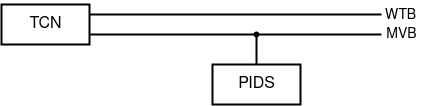
\includegraphics[width=1\textwidth]{./Figures/diagTcnPidsBusesWtbMvb.png}
	\caption{}
	\label{fig:diagTcnPidsBuusesWtbMvb}
\end{figure}


\begin{figure}[ht]
	\centering
	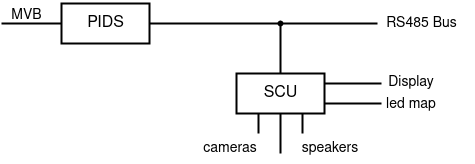
\includegraphics[width=1\textwidth]{./Figures/diagPidsScuDevices.png}
	\caption{}
	\label{fig:diagPidsScuDevices}
\end{figure}

\begin{figure}[ht]
	\centering
	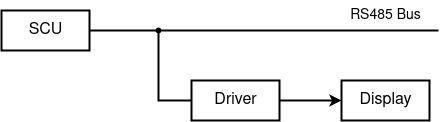
\includegraphics[width=1\textwidth]{./Figures/diagScuDriverDisplay.png}
	\caption{}
	\label{fig:diagScuDriverDisplay}
\end{figure}

\pagebreak
\subsection{Diseño}

\begin{figure}[ht]
	\centering
	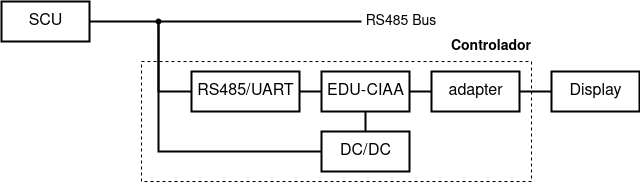
\includegraphics[width=1\textwidth]{./Figures/diagVistaReDisenhoEduCIAA.png}
	\caption{}
	\label{fig:diagVistaReDisenhoEduCIAA}
\end{figure}


\begin{figure}[ht]
	\centering
	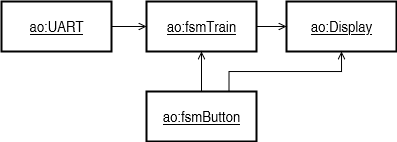
\includegraphics[width=1\textwidth]{./Figures/diagVistaDisenho.png}
	\caption{}
	\label{fig:diagVistaDisenho}
\end{figure}

\begin{figure}[ht]
	\centering
	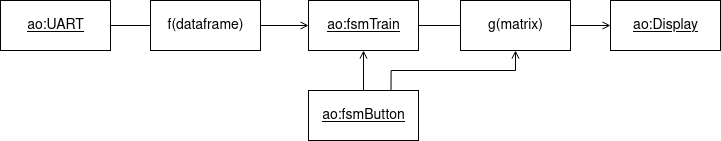
\includegraphics[width=1\textwidth]{./Figures/diagVistaDisenhoExtendida.png}
	\caption{}
	\label{fig:diagVistaDisenhoExtendida}
\end{figure}




\pagebreak
\section{Patrones}


\begin{figure}[ht]
	\centering
	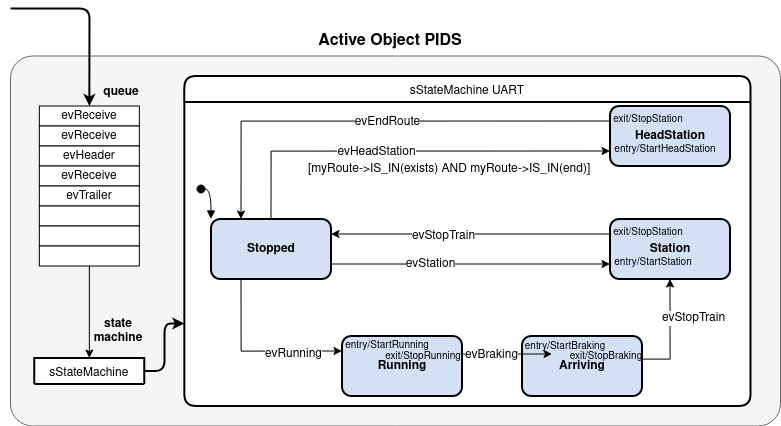
\includegraphics[width=1\textwidth]{./Figures/fsmTrain.png}
	\caption{}
	\label{fig:fsmTrain}
\end{figure}

\pagebreak
\section{Firmware}


\begin{figure}[ht]
	\centering
	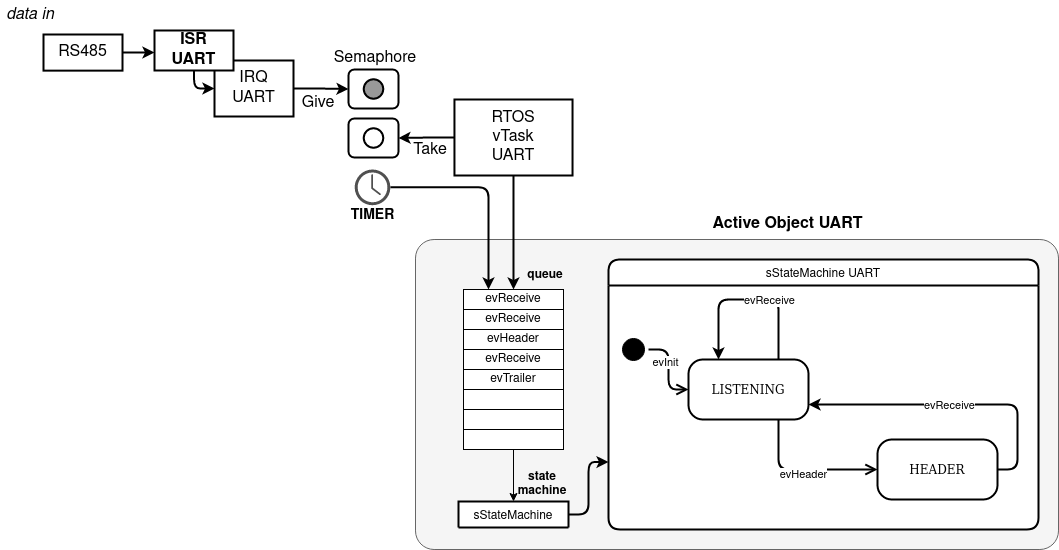
\includegraphics[width=1\textwidth]{./Figures/fsmUART.png}
	\caption{}
	\label{fig:fsmUART}
\end{figure}


\begin{figure}[ht]
	\centering
	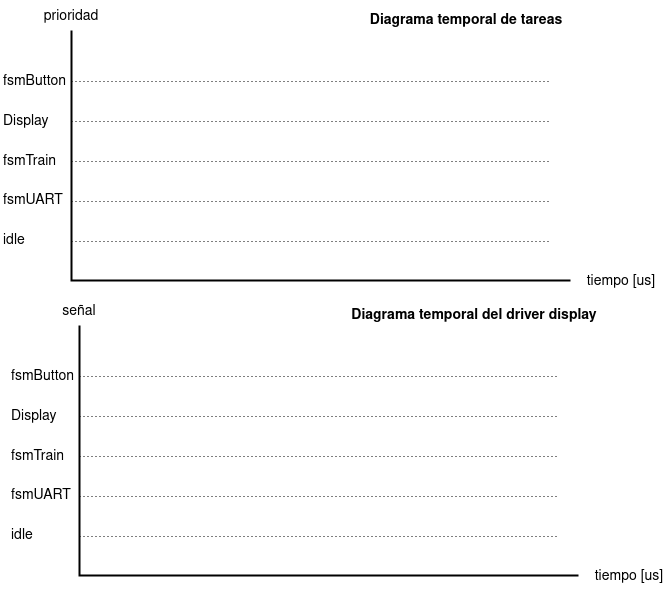
\includegraphics[width=1\textwidth]{./Figures/diagramasTemporales.png}
	\caption{}
	\label{fig:diagramasTemporales}
\end{figure}

\pagebreak
\section{Hardware}

\begin{figure}[ht]
	\centering
	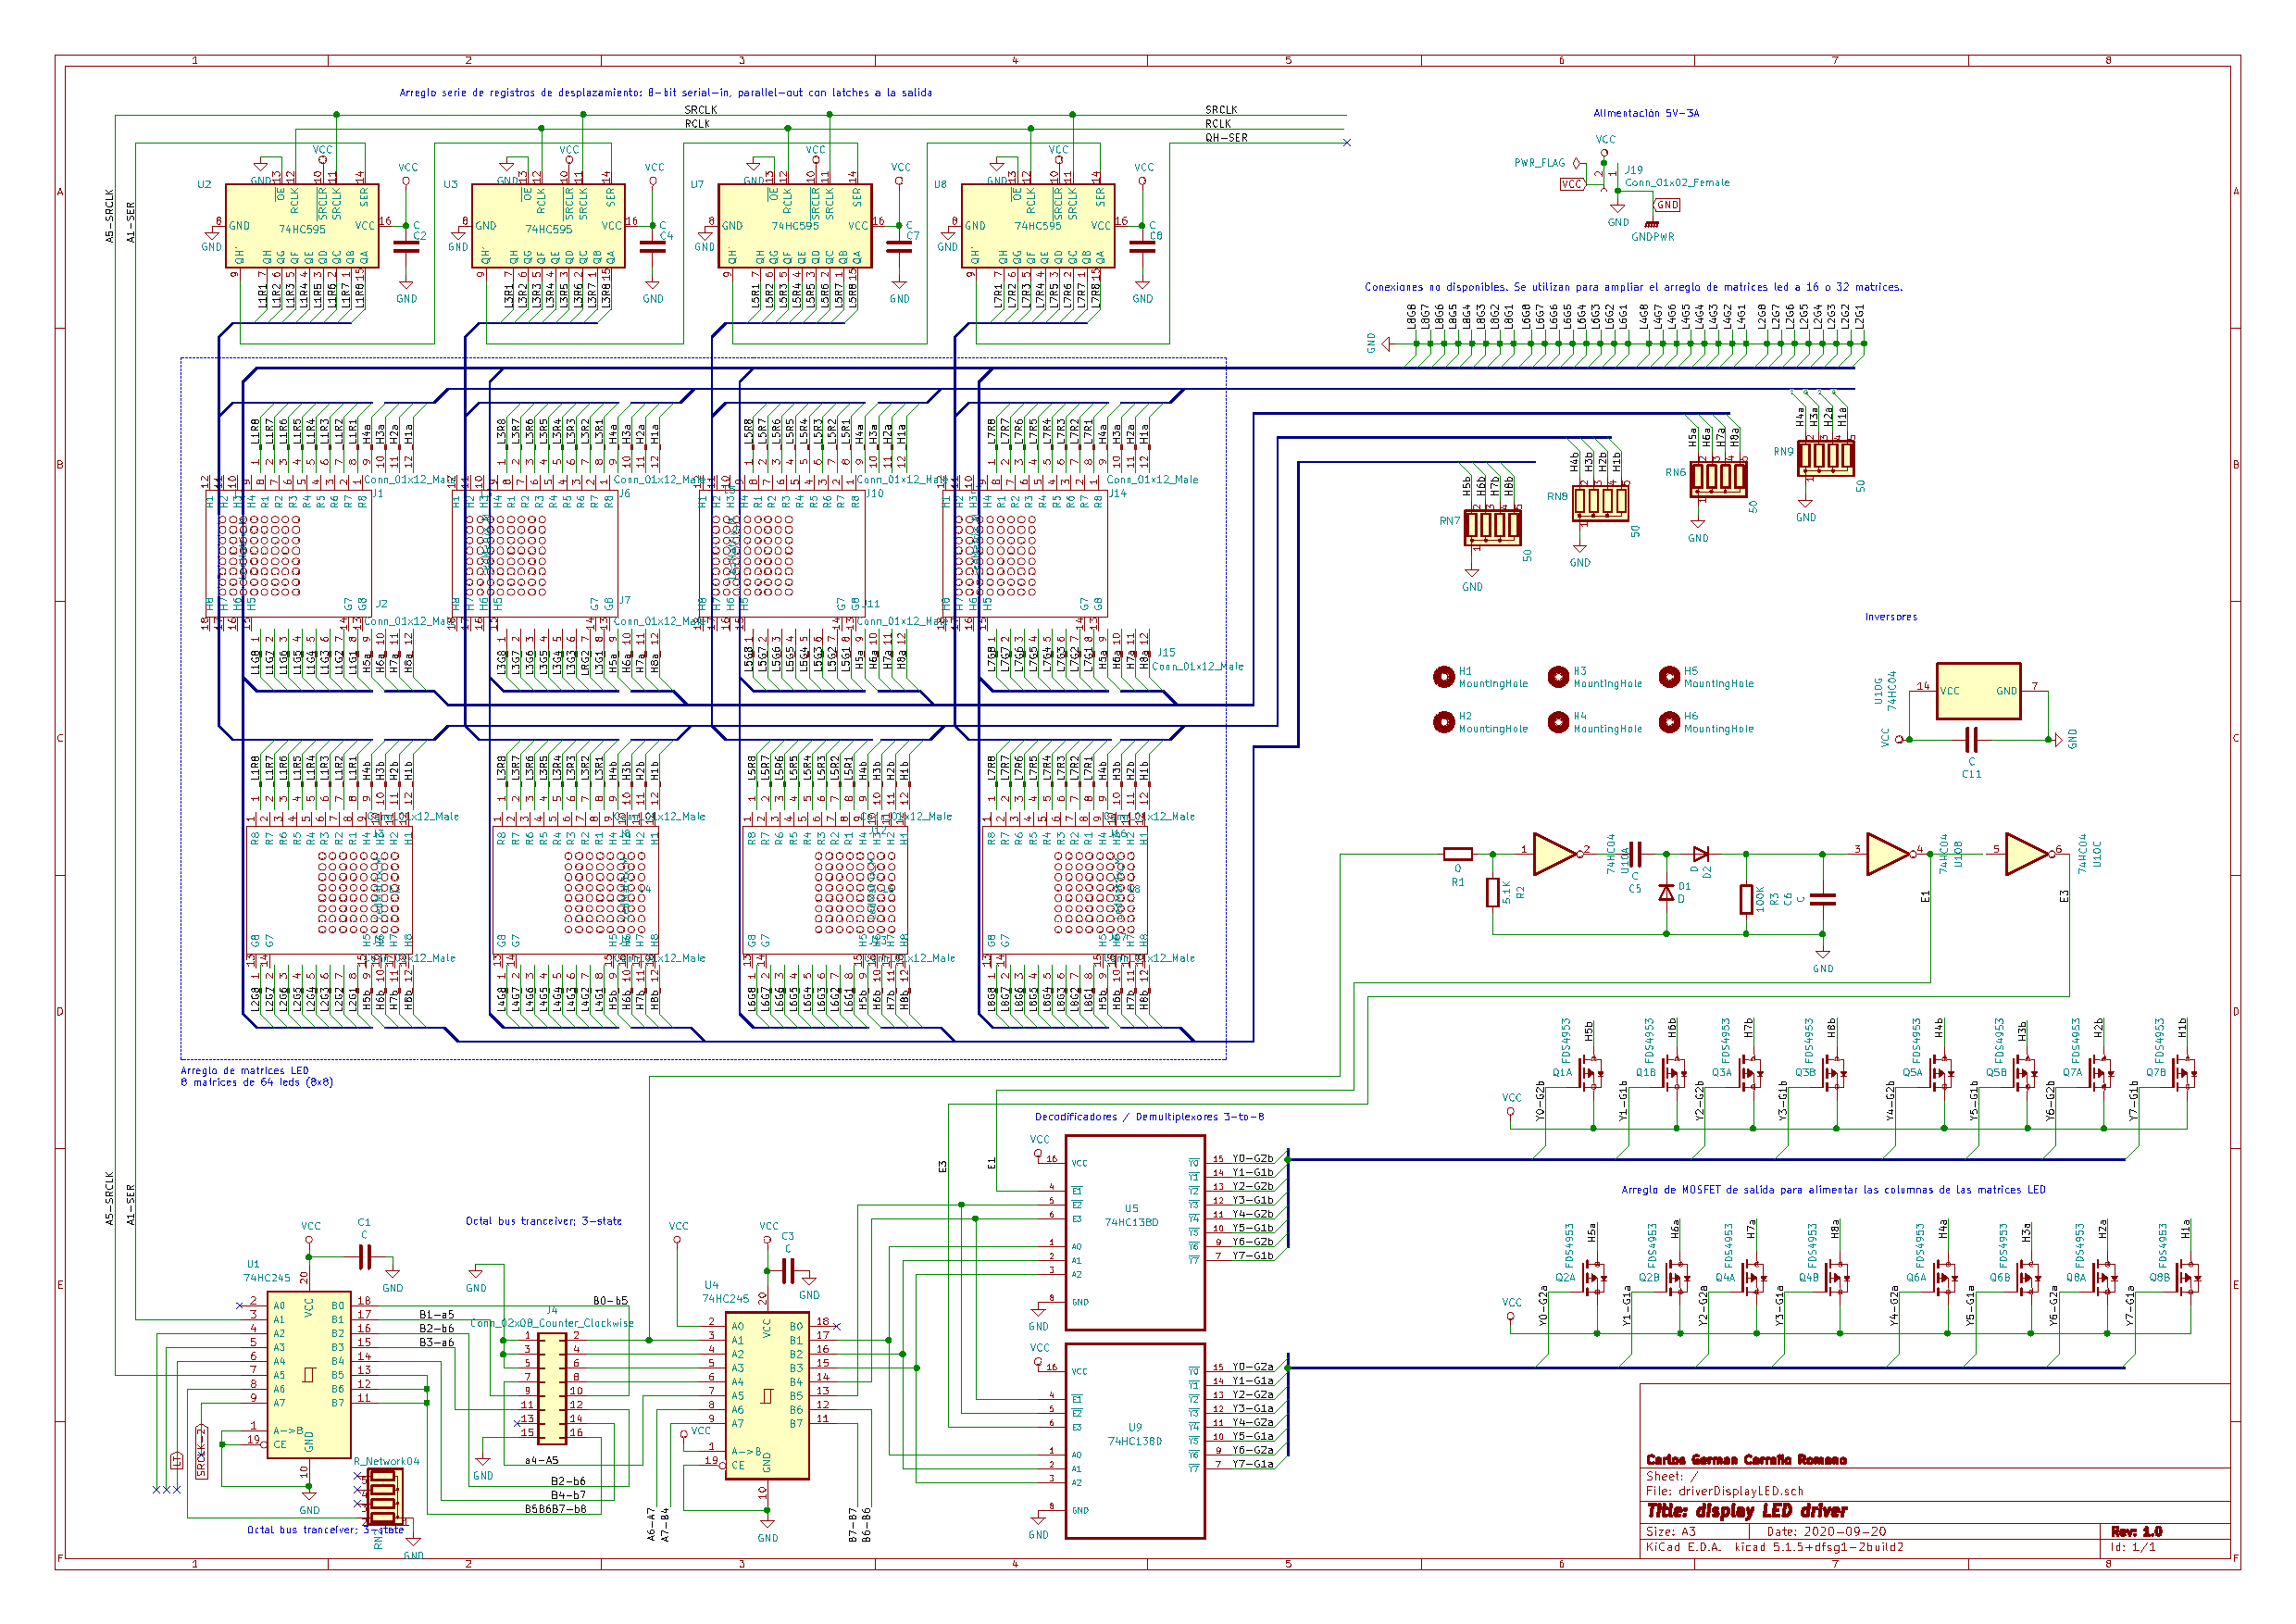
\includegraphics[width=1\textwidth]{./Figures/output.driverLED.pdf}
	\caption{}
	\label{fig:schDriverLED}
\end{figure}

\begin{figure}[ht]
	\centering
	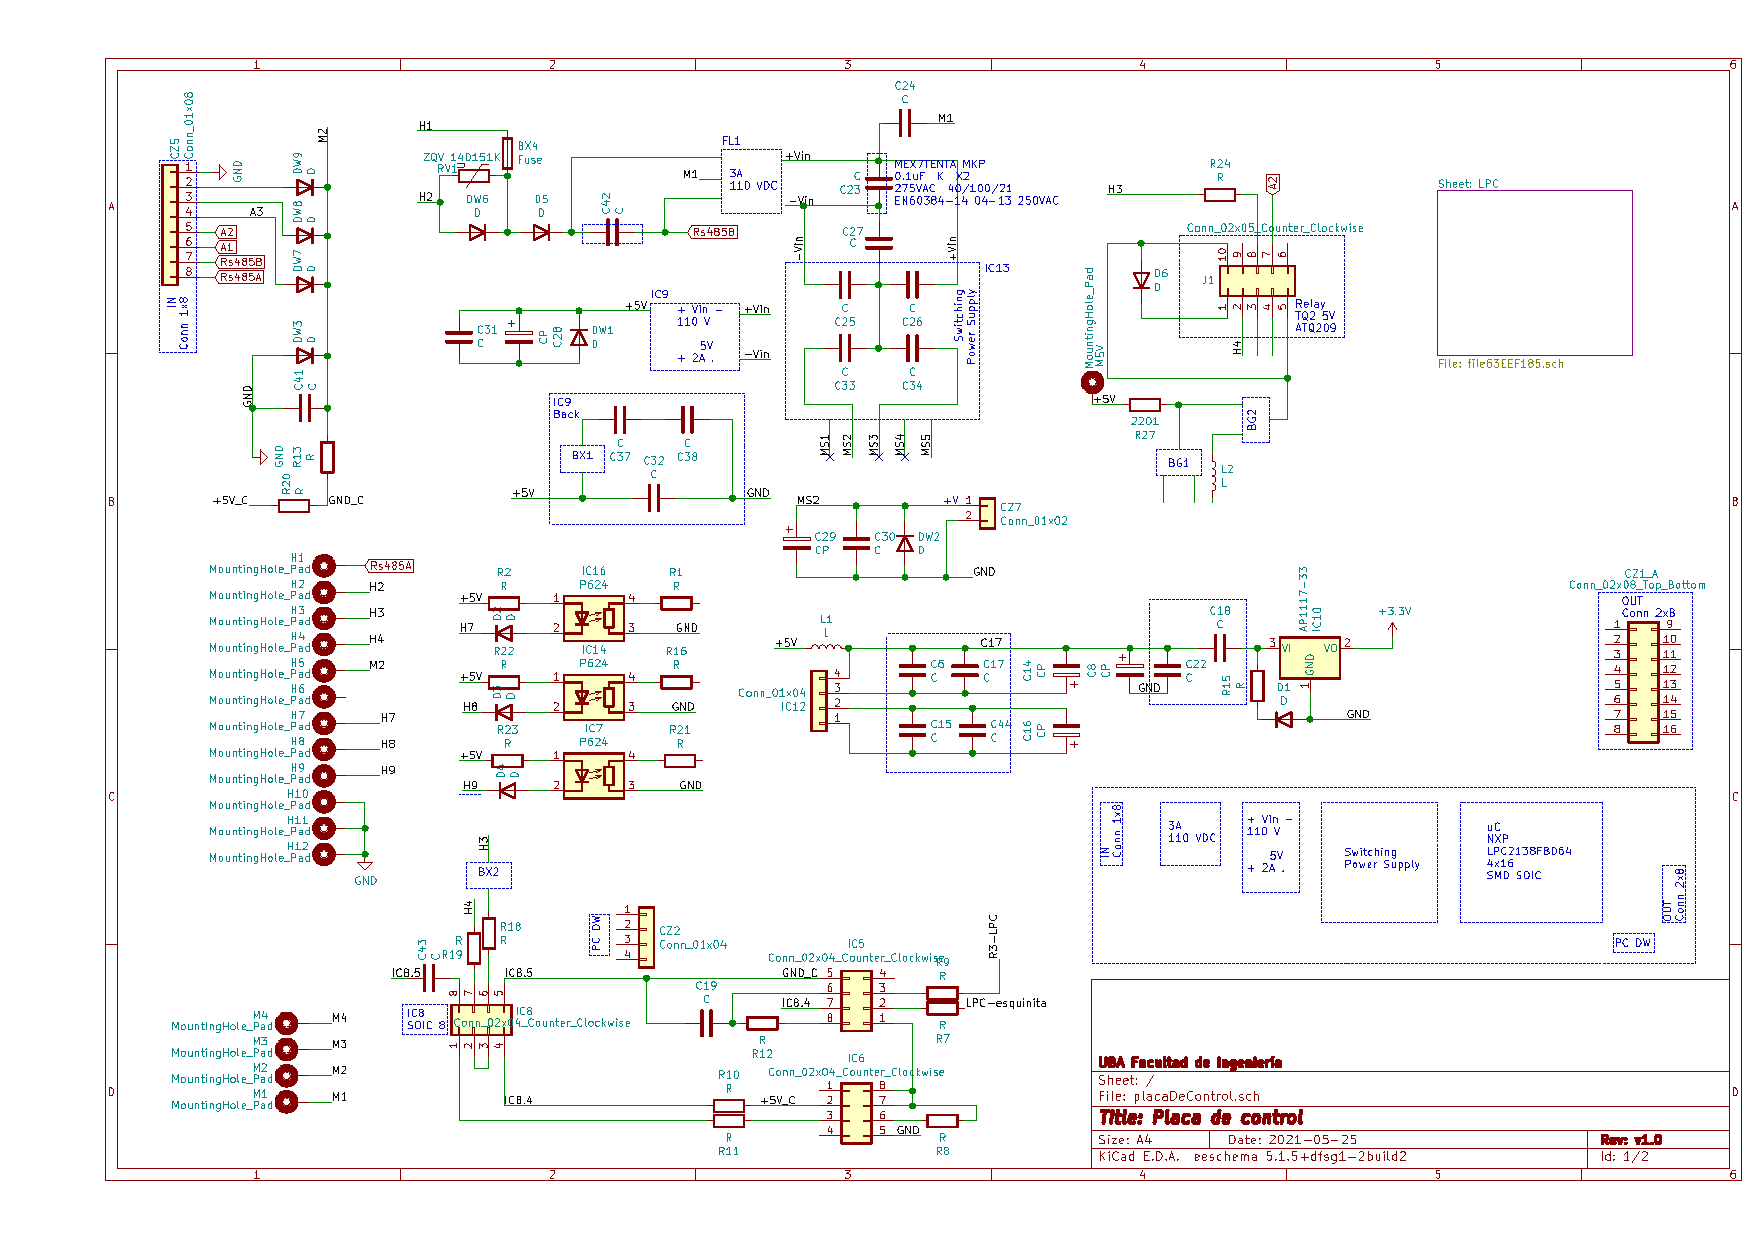
\includegraphics[width=1\textwidth]{./Figures/output.placaControl.pdf}
	\caption{}
	\label{fig:schController}
\end{figure}